\par Many computational problems in science and engineering are modeled via solving partial differential equations (PDEs) and are used to model physical phenomena such as fluid dynamics \cite{Isom_H._2008}, electricity \cite{M.Sadiku_1990}, magnetism \cite{H.Berestycki_2002}, mechanics \cite{A.Selvadurai_2000}, optics \cite{C.Tang_2013}, and heat flow \cite{rocca2015entropic}. Some of these problems can not be solved for an \gls{Analytic expression} and must rely on \gls{Numerical analysis} to generate a final answer. Numerically derived solutions are commonly solved by first discretizing them into finite difference equations or finite elements through the use of the \gls{finite difference method}. Iterative methods such as \gls{Conjugate gradient method} or the adaptive \gls{Multigrid method} are also often adopted in order to solve these equations \cite{richter2015memristive}. Due to the large number of iterations in the recursive process required to attain more accurate solutions.

\par Due to the computational energy and time expense required to solve these equations techniques have been invented to simplify their calculation, such as transforming the \acrshort{pde}s into ordinary differential equations \gls{ordinary differential equation} (\acrshort{ode}s) and much attention has been paid to creating efficient implementations of \acrshort{pde} solvers aimed at reducing the number of iterations \cite{J.Zhu_1994, L.Pinuel_1998}. A \acrshort{pde} solution of heat flow over a homogeneous surface computed numerically requires the decomposition of the surface into an array of subsurfaces through the finite difference method, known as a computational mesh.  Subsurfaces with smaller areas yield higher-precision results, but require more computations to arrive at a solution. As PDEs form the basis for many applications in scientific computing, efficiencies gained in this domain would be of great benefit to the scientific community \cite{J.Dongarra_2017}.

\par The analog alternative to this digitally implemented numerical method traditionally utilized analogue circuits comprised of Resistor(R), Inductor(L), and Capacitor (C) elements that bypass the iterative recursive process by generating a mesh based solution in a single execution, equivalent to a computational complexity \gls{Big O notation} of 1 or $n$ (linear) depending on the speed of execution, once boundary conditions for the problem are set within the mesh, with the accuracy of the solution being determined by combination of the density of the mesh utilized and the area of the problem being solved for. This electrical analog finite difference architecture utilizes summation of current for computation and  was originally developed to provide efficient computation of heat transfer \cite{G.Liebmann_1950} and oscillatory flow problems in aeronautical engineering \cite{P.Palmer_1959}, and has been shown to reduce the time to solution through its elimination of the iterative processing steps which retard numerical methods.

Solving \acrshort{pde}s using Electrical Analogues requires an array of circuit elements suitably connected in order to yield electrical analogue of a PDE. A two-dimensional resistor array can generate an analog solution to a Laplace equation,

\begin{equation}\label{Laplace}
\nabla^2 \varphi = 0
\end{equation}
\nomenclature[A]{$\nabla^2$}{Laplace operator}
\nomenclature[A]{$\varphi$}{A twice-differentiable real-valued function}

while sampling current at nodes, we expand the class of PDEs to non zero solution Poisson Equations,

\begin{equation}\label{Poisson}
\nabla^2 \varphi = ki
\end{equation}
\nomenclature[A]{$ki$}{Real or complex-valued function on a manifold}

with the addition of capacitors at at nodes, we account for time dependence and expand the class of \acrshort{pde}s to Diffusion Equations,

\begin{equation}\label{Diffusion}
\nabla^2 \varphi = k \frac{\partial \varphi}{\partial t }
\end{equation}

and by substituting capacitors for resistors and keeping capacitors at nodes, we expand the class of \acrshort{pde}s to Wave Equations,

\begin{equation}\label{Wave}
\nabla^2 \varphi = k \frac{\partial^2 \varphi}{\partial t^2}
\end{equation}

These classes of PDEs that can be accelerated by an electronic analog mesh based co-processor each solve problems in a specific application-space and cater to a wide spectrum of the standard simulation applications in science and engineering. 

\begin{figure}[ht]
    \centering\fbox{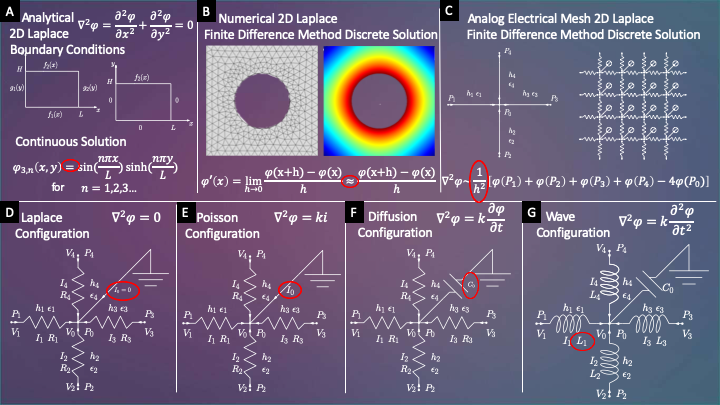
\includegraphics[height=3in, width=5.5in]{figures/figures1/01_analytical_numerical_analog.png}}
    \caption{The top row of this figure illustrates the traditional options available for solving a PDE through \textbf{(A)} analytical, \textbf{(B)} numerical, and \textbf{(C)} analog electrical PDE solving paradigms, while the bottom row illustrates the reconfigurations of an analog electrical discrete solution for different classes of \acrfull{pde}s including \textbf{(D)} Laplace, \textbf{(E)} Poisson, \textbf{(F)} diffusion, and \textbf{(G)} wave equation.}
    \label{fig:01_analytical_numerical_analog}
\end{figure}

Due to complexities surrounding the effective integration of a static analog mesh computer in a \acrfull{vlsi} architecture, the resistance network analogue has remained in the academic domain \cite{J.Ramirez-Angulo_2000}. This shortcoming was improved upon by Ramirez-Angulo and DeYong \cite{J.Ramirez-Angulo_2000} with a VLSI-friendly implementation of an analog mesh computer using Complementary Metal Oxide Semiconductor (CMOS) transistors operated in the subthreshold regime.  However, modern digital VLSI designs prefer the use of minimum-size devices, which is at odds with subthreshold CMOS designs, which require larger devices to ensure proper matching \cite{A.Hastings_2005}.  

\par Recent programs advocating for new and innovative computer architectures \cite{darpa2017}, and the recent introduction of innovative, programmable VLSI devices, such as the nanophotonic modulator \cite{V.Sorger_2012}, have created opportunities for innovative architectures that can take advantage of these new devices \cite{A.Mehrabia_2018,S.Sun_2018}. Conceptual metastructure based analog computing models are starting to be developed by leaders in the field including Nader Engheta \cite{Mohammadi_Estakhri1333}.  In the telecommunications space, Photonic ROC can potentially be used to efficiently model \gls{multiple-input and multiple-output} (\acrshort{mimo}) systems that make substantial use of \acrshort{pde}s \cite{tsoulos2006mimo}. The recent push for \gls{post-Moore} computer architectures \cite{darpa2017}, has introduced a wide variety of application-specific accelerators \cite{hu2016dot,bojnordi2016memristive,J.George_2017}.  Generally, these accelerators are designed to improve the performance of computationally-intensive algorithms by limiting unnecessary calculations or data movements. To maximize an application-specific computer's utility, it must be capable of accelerating widely used algorithms. The progression to an analog electrical \acrshort{pde} solution accelerator is shown in Figure \ref{fig:01_analytical_numerical_analog}.
